% !TEX root = ../main.tex
\subsection{Validation and Results} \label{ssec::validationandresults}
% --+ Data used +---------------------------------------------------------------
    Just as with the residuals validation, the results presented in this document are based on the application of this work on RG-F data.
    It's worth noting that the RG-F target is $\sim60$ centimetres long, much larger than the average CLAS12 target \cite{hattawy2019}.
    In particular, the runs used for testing and validation are presented in table \ref{tab::rgf_data}, and the run used to obtain the data displayed in this section was $\mathbf{011983}$.

    \begin{table}[h!]
        \centering
        \begin{tabular}{c|llll}
            \textbf{Run Number} & \textbf{Energy (MeV)} & \textbf{Current (nA)} & \textbf{Configuration} & \textbf{Target} \\
            \hline
            \textbf{011983}     & 10389.4 &  50 & Inbending & D2 \\
            \textbf{012016}     & 10389.4 & 250 & Inbending & D2 \\
            \textbf{012439}     &  2186.4 &  15 & Inbending & H2 \\
            \textbf{012461}     & 10196.6 &  20 & Inbending & D2
        \end{tabular}
        \caption{RG-F runs used for validation.}
        \label{tab::rgf_data}
    \end{table}

% --+ Cuts +--------------------------------------------------------------------
    Some additional cuts are applied to the tracks to obtain the plots presented in this section.
    These cuts are merely to remove very bad tracks which would nonetheless not be used in analysis.
    \begin{itemize}
        \item \texttt{abs(chi2pid) < 5}: Remove tracks without enough certainty on the PID of a particle.
        \item \texttt{vz < fmtZ}: Remove tracks further downstream than FMT.
        \item \texttt{chi2/ndf < 15}: Don't use tracks with too much uncertainty.
    \end{itemize}

% --+ Geometry issue +----------------------------------------------------------
    To measure the improvement in vertex resolution, we'll compare the vertex position of tracks that passed only through DC reconstruction and tracks that passed through both DC and FMT reconstruction.
    For simplicity, we'll refer to the former as DC tracks and the latter as FMT tracks.
    Remembering that the $z$ axis is concentric with the beamline, figure \ref{fig::dc_vs_fmt_vz} shows the vertex $z$ position of DC tracks versus that of FMT tracks.

    \begin{figure}[h!]
        \centering\frame{
        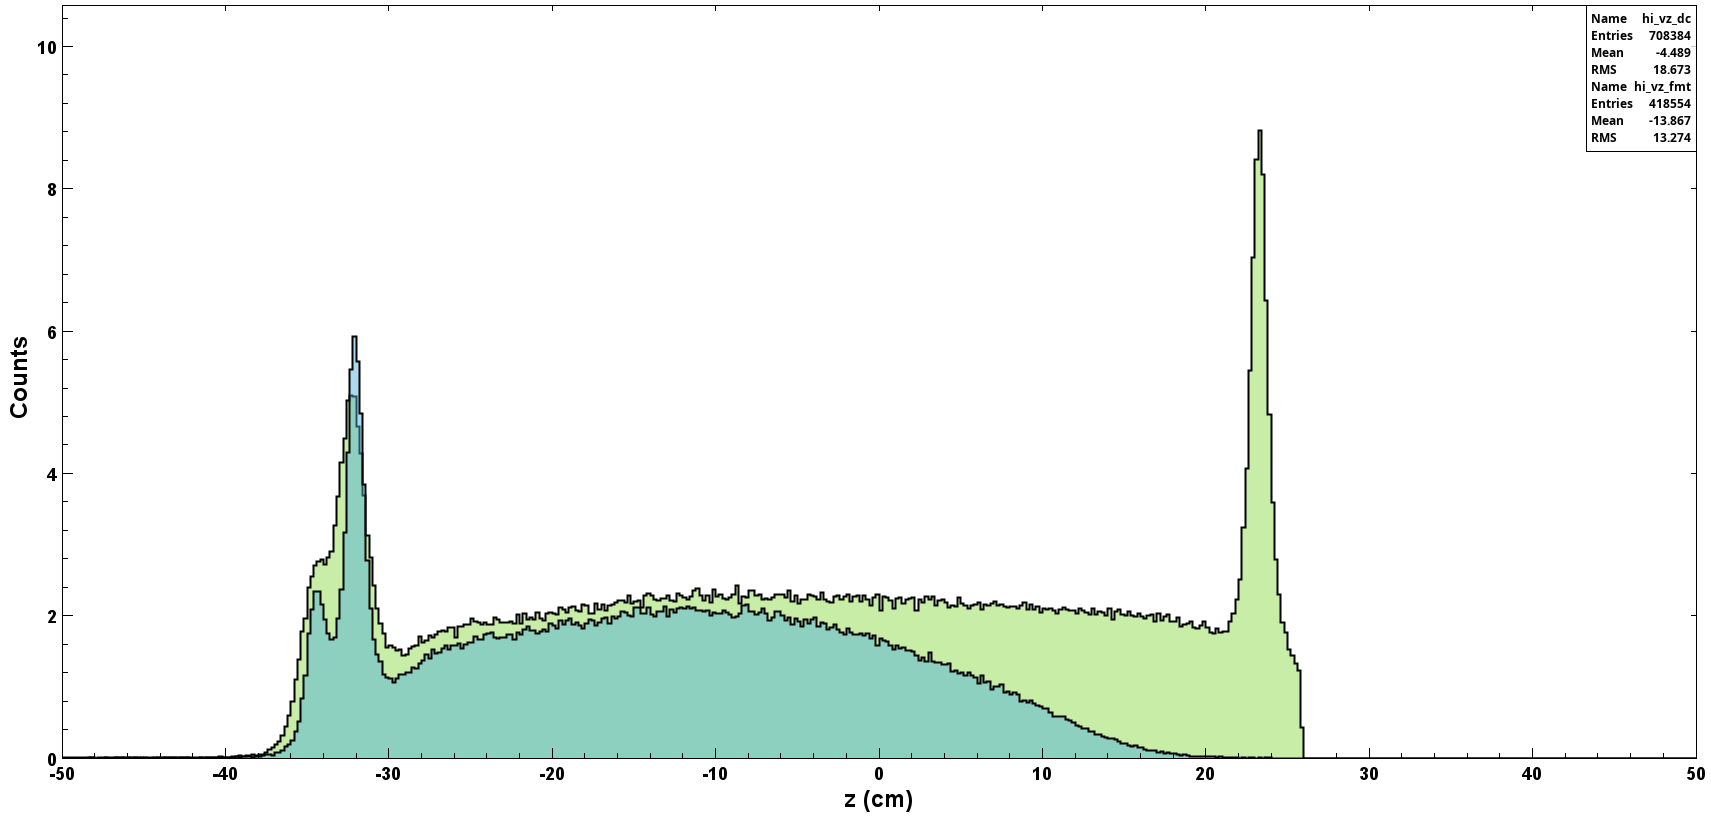
\includegraphics[width=\textwidth]{12fmtalign/img/40dc_vs_fmt.png}}
        \caption[DC vs FMT $z$ without geometric correction]{DC vs FMT vertex $z$ for electrons without any geometric correction. DC tracks are shown in green while FMT tracks are shown in blue. Note that the dark cyan colour comes from the overlap.}
        \label{fig::dc_vs_fmt_vz}
    \end{figure}

    To understand the plot in the figure, it's worthwhile to take a minute to look at the RG-F target.
    The target itself is a large chamber filled with gas, with a composition that changes across runs.
    The distance between the windows of the chamber is of $553.32$ millimetres.
    In addition, it was found that the upstream window of the target is separated by about $24$ millimetres from the beam window.
    % This is a far cry from the nominal distance, which was expected to be of $9.16$ millimetres.
    All windows are made of aluminium and have a thickness of $15$ micrometres. % TODO. CITATION PENDING.
    A detailed drawing of the target can be seen in addendum 1.

    From figure \ref{fig::dc_vs_fmt_vz}, it is immediately obvious that the FMT detector only recognises the upstream windows, completely missing the downstream one.
    This is purely a geometric issue:
    the downstream window is outside of the FMT active detection area.
    The effect is easy to see in figure \ref{fig::vz_vs_theta}, where the vertex $z$ coordinate is plotted against the $\theta$ angle.
    The two red lines in the plots show FMT's active area, and the downstream windows is clearly outside of it, hence why it disappears.

    \begin{figure}[t!]
        \centering\frame{
        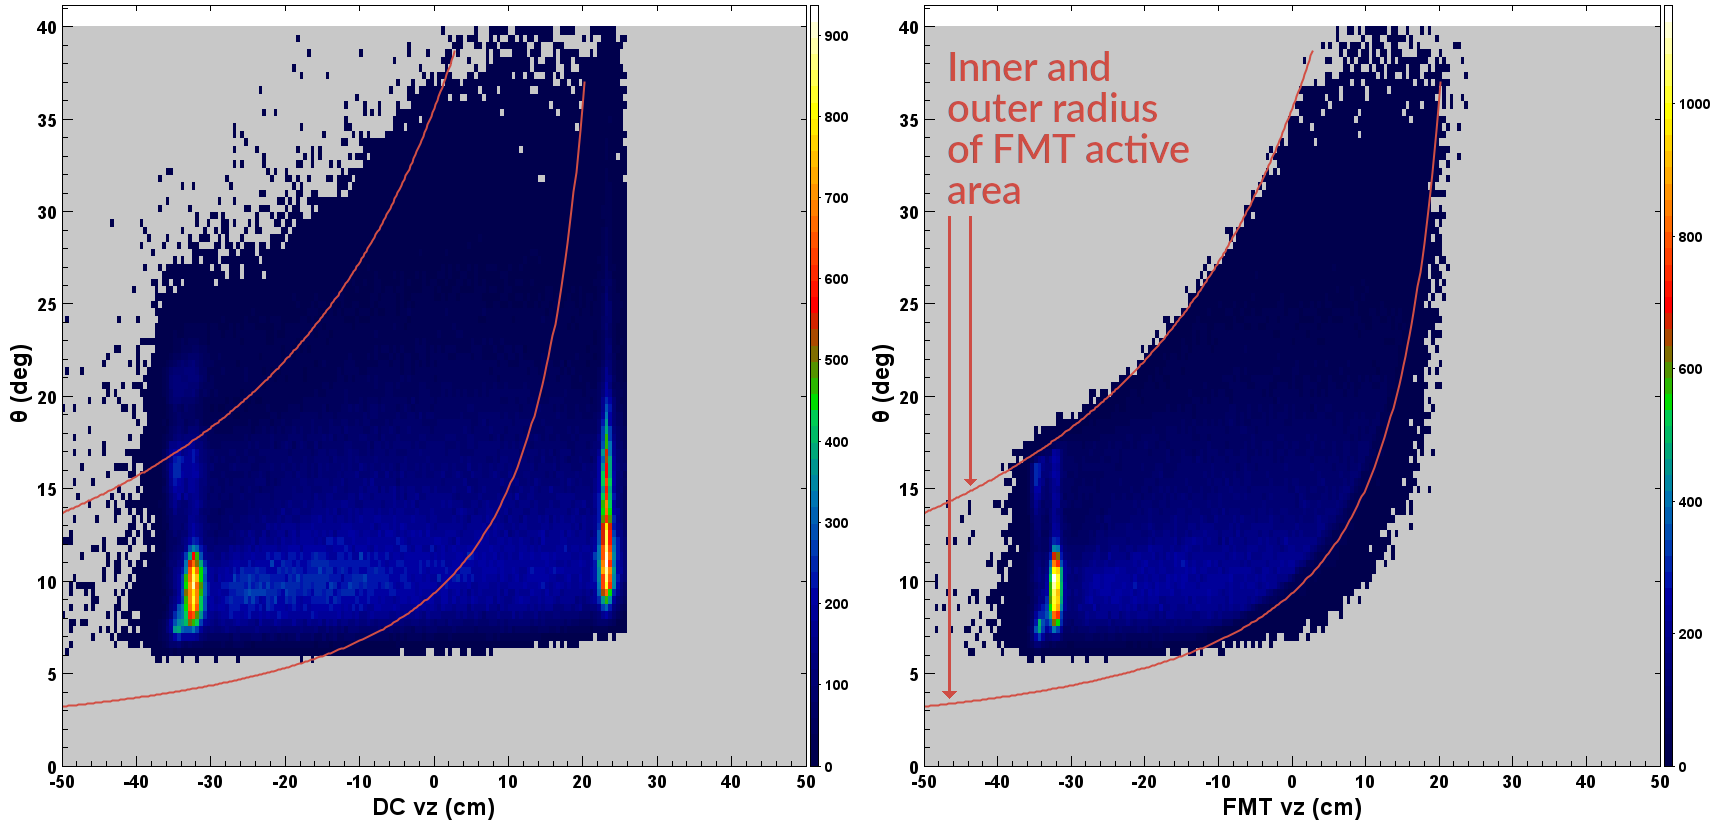
\includegraphics[scale=0.24]{12fmtalign/img/40theta_dc_vs_fmt.png}}
        \caption[$z$ vs $\theta$ for DC and FMT.]{$z$ vs $\theta$ for DC and FMT for electrons without any geometry correction. FMT's active area are shown in red lines.}
        \label{fig::vz_vs_theta}
    \end{figure}

    To account for this geometric effect, we apply an additional cut based on the plotted curves.
    The curves are given by
    \begin{equation*}
        c_1 = 57.29 \cdot \arctan\left(\frac{r_\text{inner}}{z_0 - z}\right), \hspace{0.5cm}
        c_2 = 57.29 \cdot \arctan\left(\frac{r_\text{outer}}{z_0 - z}\right),
    \end{equation*}
    where $r_\text{inner}$ is the radius of the hole at the center of FMT, $r_\text{outer}$ is the radius of the outer circumference of FMT, and $z_0$ is the $z$ position of the first FMT layer plus the drift distance.
    All these parameters are read from the CCDB.

% --+ Show vertex position resolution improvement +-----------------------------
    In addition, one final cut was added.
    At the time of writing, beam alignment is yet to be performed for RG-F data, which causes a loss in vertex resolution.
    Since this hampers the accuracy of reconstruction, we added an additional cut to only use one sector of the detector.

    \begin{figure}[b!]
        \centering\frame{
        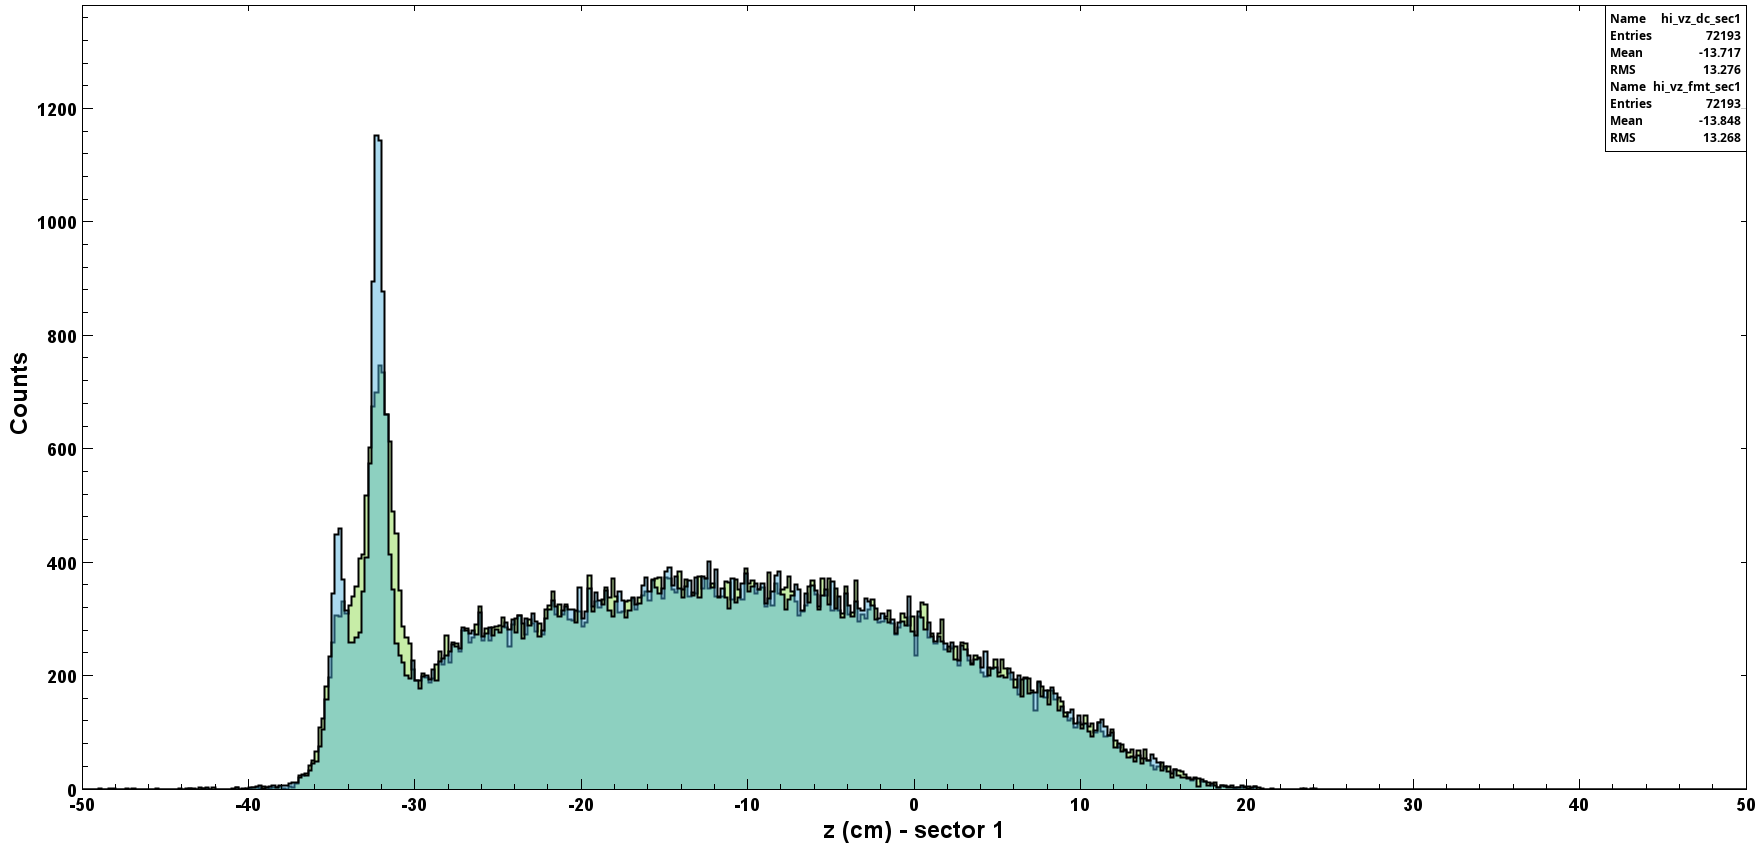
\includegraphics[scale=0.24]{12fmtalign/img/40dc_vs_fmt_sector1.png}}
        \caption[DC vs FMT $z$ with geometry correction]{DC vs FMT vertex $z$ for electrons with a geometric correction. DC tracks are shown in green while FMT tracks are shown in blue. Data from only one CLAS12 sector was used to obtain this plot.}
        \label{fig::dc_vs_fmt_vz_corrected}
    \end{figure}

    The resolution plot contrasting DC and FMT tracks using all the cuts referred up to this point can be seen in figure \ref{fig::dc_vs_fmt_vz_corrected}.
    To measure both DC and FMT resolution, we'll use two Gaussian curves compounded with a quadratic curve to account for the background.
    The fit is defined as
    \begin{equation*}
        \text{amp}_1 \cdot \text{gaus}(z, z_\text{max}, \sigma) + \text{amp}_2 \cdot \text{gaus}(z, z_\text{max} - 2.4, \sigma) + p_1 + p_2\cdot z + p_3\cdot z^2,
    \end{equation*}
    where $\text{amp}_1$ is the amplitude of the biggest peak and $z_\text{max}$ is its $z$ position, $\text{amp}_2$ is the amplitude of the leftward peak, whose position was measured to be $2.4$ centimetres, and all the other parameters are obtained by fitting.

% --+ Resolution for electrons +------------------------------------------------
    % TODO. Update with plots from rge-analysis.
    For electrons in run \textbf{011983} (low luminosity, $50$ nA), this gives a DC resolution of $\sigma_\text{DC} = 0.875$ cm and an FMT resolution of $\sigma_\text{FMT} = 0.387$ cm --- a doubling in resolution.
    For electrons in run \textbf{012016} (production luminosity, $250$ nA), this gives a DC resolution of $\sigma_\text{DC} = 1.009$ cm and an FMT resolution of $\sigma_\text{FMT} = 0.596$ cm.

% --+ Resolution with no particle cuts +----------------------------------------
    % TODO. Update with plots from rge-analysis.

% --+ Conclusions +-------------------------------------------------------------
    While the improvement in resolution is less than what was originally predicted for the detector, it is still a very encouraging result.
    The increase in resolution allows for more precise target position measurements.
    This, for example, allows for double targets to be placed closer to each other, benefiting the physics derived from such experiments, such as the RG-E run. % TODO. CITATION NEEDED.

    The reason behind the improvement not being as large as predicted is attributed to the fact that the original projection considered six FMT layers.
    This amount of layers would add more position data in the particle's track, allowing the fitting process to better measure its vertex position.

% --+ Why no improvements is seen on vertex momentum resolution +---------------
    In addition, the lack of more layers and the proximity between them means that FMT has a small lever arm.
    This means that the detector cannot provide a good contribution to the vertex momentum resolution, since there is not enough data added to the track's momentum. % TODO. MAYBE CITATION NEEDED?

% --+ Show detector efficiency +------------------------------------------------
    Finally, in the interest of understanding the FMT detector, we briefly study the efficiency of FMT.
    We define efficiency as the number of FMT tracks divided by the number of DC tracks or, in other words, how many of the DC tracks were detected by FMT as well.
    With the three layer configuration, efficiency is $\sim 88.96\%$.
    As can be seen in figure \ref{fig::fmt_efficiency}, there is no anomalous geometric effect in layer-by-layer efficiency.
    The gaps seen are merely due to the geometry of CLAS12, since its separated into six sectors.

    \begin{figure}[b]
        \centering\frame{
        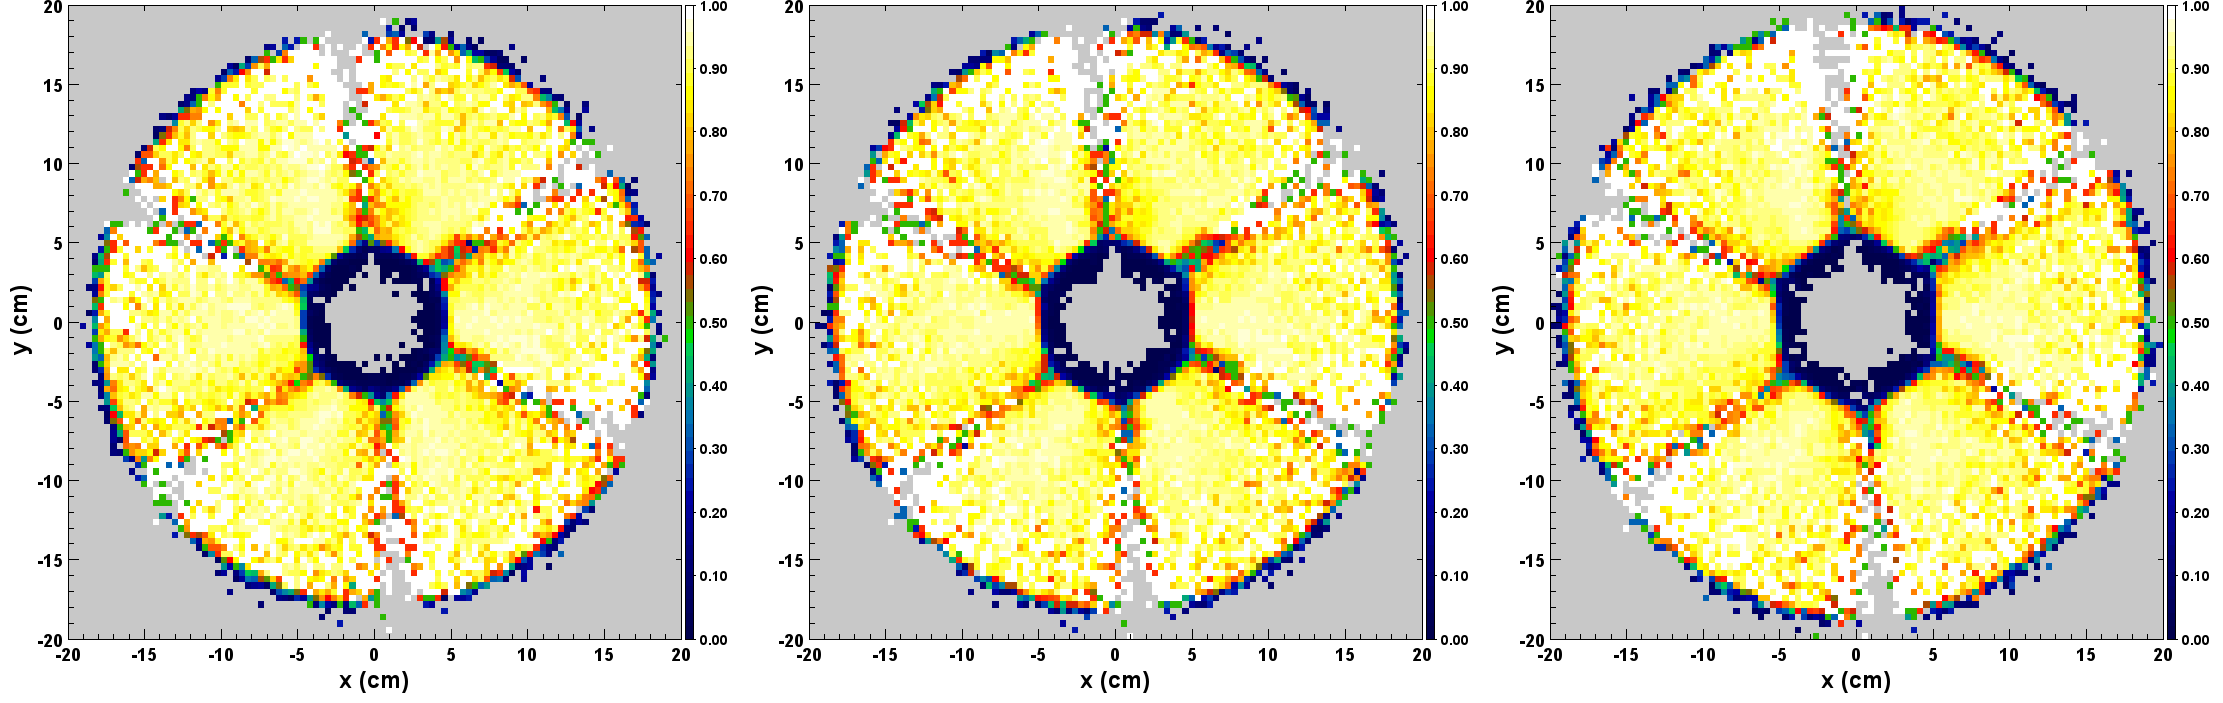
\includegraphics[width=\textwidth]{12fmtalign/img/40fmt_efficiency.png}}
        \caption[FMT layers efficiency]{Efficiency of each FMT layer.}
        \label{fig::fmt_efficiency}
    \end{figure}
